\documentclass[journal]{IEEEtran}
\usepackage{graphicx}
\usepackage{amsmath}
\usepackage{hyperref}
\usepackage{float}
\usepackage{subcaption}
\usepackage{booktabs}
\usepackage{pgfplotstable}
\usepackage{qrcode}

\pgfplotsset{compat=1.18}

\begin{document}

% Cover Page
\begin{titlepage}
    \centering
    
\includegraphics[width=0.2\textwidth]{IMAGES/university_logo.png}\\[1cm]
    
    \Large
    Istanbul University\\
    Department of Physics\\[0.5cm]
    
    \rule{\linewidth}{0.2mm} \\[0.4cm]
    
    \Huge
    \textbf{Analysis of RL and RC Circuits}\\[0.4cm]
    
    \rule{\linewidth}{0.2mm} \\[1.5cm]
    
    \Large
    \textbf{IBRAHIM H.I. ABUSHAWISH}\\[2cm]
    
    \large
    \begin{tabular}{ll}
        Student ID: & 0412230047 \\[0.3cm]
        Instructor: & Lect. Deniz BOZOĞLU PARTO \\[0.3cm]
        Experiment Date: & December 16, 2024 \\[0.3cm]
        Report Submission Date: & December 23, 2024 \\[0.3cm]
        Course Title and Section: & PHYS2305 \\[1cm]
    \end{tabular}
    
    \vfill
\end{titlepage}

% \tableofcontents

% \listoffigures
% \listoftables

\pgfplotsset{compat=1.18}

\begin{abstract}
This report presents a comprehensive analysis of RL and RC circuits. It provides a detailed theoretical overview, experimental procedures, data analysis, and discussion of key findings. The analysis is supported by calculations and graphical visualizations. Key conclusions are highlighted, particularly on the behavior of the circuits under varying resistance and capacitance settings.
\end{abstract}

\begin{IEEEkeywords}
RL Circuit, RC Circuit, Time Constant, Frequency Response
\end{IEEEkeywords}

% Introduction 
\section{Introduction}
This section introduces the concepts of RL and RC circuits. The primary aim is to investigate the behavior of these circuits under different conditions. Understanding these circuits is critical in analyzing the transient and steady-state responses in electrical systems.

% Theoretical Background
\section{Theoretical Background}
In this section introduces the equations used in the analysis of RL and RC circuits, as provided in the lab manual \cite{lab_manual}.

\subsection{RL Circuit}
An RL circuit consists of a resistor (R) and an inductor (L) connected in series or parallel. The behavior of the circuit is governed by the differential equation:
\begin{equation}
    V(t) = L \frac{dI(t)}{dt} + IR \label{eq:rl_voltage}
\end{equation}
where \(V(t)\) is the voltage, \(I(t)\) is the current, \(L\) is the inductance, and \(R\) is the resistance.

The impedance \(Z\) of the RL circuit is given by:
\begin{equation}
    Z = \sqrt{R^2 + (\omega L)^2} \label{eq:rl_impedance}
\end{equation}
where \(\omega\) is the angular frequency of the AC source.

The phase angle \(\phi\) between the voltage and the current is:
\begin{equation}
    \phi = \arctan\left(\frac{\omega L}{R}\right) \label{eq:rl_phase}
\end{equation}

\subsection{RC Circuit}
An RC circuit consists of a resistor (R) and a capacitor (C) connected in series or parallel. The behavior of the circuit is governed by the differential equation:
\begin{equation}
    V(t) = IR + \frac{1}{C} \int I(t) dt \label{eq:rc_voltage}
\end{equation}
where \(V(t)\) is the voltage, \(I(t)\) is the current, \(R\) is the resistance, and \(C\) is the capacitance.

The impedance \(Z\) of the RC circuit is given by:
\begin{equation}
    Z = \sqrt{R^2 + \left(\frac{1}{\omega C}\right)^2} \label{eq:rc_impedance}
\end{equation}

The phase angle \(\phi_{RC}\) between the voltage and the current is:
\begin{equation}
    \phi_{RC} = \arctan\left(-\frac{1}{\omega RC}\right) \label{eq:rc_phase}
\end{equation}

These equations form the basis for the calculations performed in the experiment, as detailed in the Jupyter notebook `Calculations.ipynb`. The notebook includes the computation of various physical quantities such as impedance, phase angle, and component values for both RL and RC circuits.

% Experimental Setup
\section{Experimental Setup}
The experimental setup includes RL and RC circuits with variable resistors and capacitors. The primary components are:
\begin{itemize}
    \item Resistor: Variable resistor for adjusting resistance.
    \item Inductor: Inductor for RL circuit.
    \item Capacitor: Capacitor for RC circuit.
    \item Measurement devices: Multimeter and oscilloscope for measuring voltage and current.
\end{itemize}

\begin{figure}[H]
    \centering
    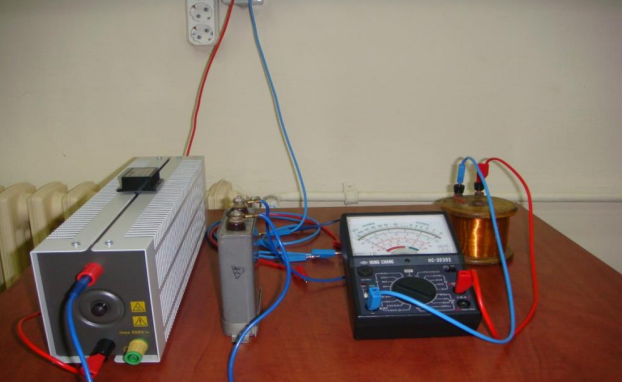
\includegraphics[width=0.8\linewidth]{IMAGES/Experimental_setup.png}
    \caption{Physical Experimental Setup with RL and RC Circuits}
    \label{fig:exp_setup}
\end{figure}
The experimental diagram is shown in Fig.~\ref{fig:exp_diagram}. This diagram provides a clear representation of the connections and components used in the experiment. It includes the RL and RC circuits, the variable resistors, the inductor, the capacitor, and the measurement devices such as the multimeter and oscilloscope. The diagram helps in understanding the setup and the flow of current and voltage in the circuits.
\begin{figure}[H]
    \centering
    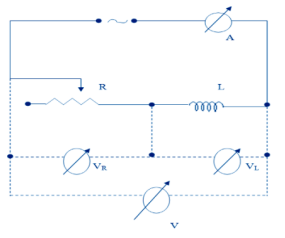
\includegraphics[width=0.8\linewidth]{IMAGES/Experimental_diagram.png}
    \caption{Schematic Diagram of the Experimental Setup}
    \label{fig:exp_diagram}
\end{figure}
% Methodology
\section{Methodology}
The experiment begins by setting up the RL and RC circuits. The resistance and capacitance are varied, and the corresponding voltage and current are measured. This process is repeated for different values to observe changes in the circuit behavior.

% Results
\section{Results}

The results of the experiment are presented in the form of calculated values for various physical quantities in the RL and RC circuits. These values are derived from the measurements and calculations performed during the experiment.

\subsection{RL Circuit}
\begin{table}[H]
    \centering
    \caption{Calculated Physical Quantities for RL Circuit}
    \label{tab:rl_results}
    \begin{tabular}{cc}
        \toprule
        \textbf{Physical Quantities} & \textbf{Calculated} \\
        \midrule
        \(i\) (A) & 0.2 \\
        \(v_R\) (V) & 43.7 \\
        \(v_L'\) (V) & 26.0 \\
        \(v\) (V) & 60.0 \\
        \(v_{RL}\) (V) & 11.5 \\
        \(v_L\) (V) & 23.0 \\
        \(L\) (H) & 0.366 \\
        \(Z\) ($\Omega$) & 299.0 \\
        \(R_L\) ($\Omega$) & 57.5 \\
        \(R\) ($\Omega$) & 218.5 \\
        $\omega$ (s$^{-1}$) & 314.159 \\
        \(\phi\) (deg) & 22.62 \\
        \(\phi_L\) (deg) & 63.43 \\
        \bottomrule
    \end{tabular}
\end{table}

\subsection{RC Circuit}
\begin{table}[H]
    \centering
    \caption{Calculated Physical Quantities for RC Circuit}
    \label{tab:rc_results}
    \begin{tabular}{cc}
        \toprule
        \textbf{Physical Quantities} & \textbf{Calculated} \\
        \midrule
        \(i\) (A) & 0.6 \\
        \(v_R\) (V) & 40.0 \\
        \(v_C\) (V) & 30.0 \\
        \(v\) (V) & 50.0 \\
        \(\omega\) ($s^{-1}$) & 314.159 \\
        \(\phi_{RC}\) (deg) & -36.87 \\
        \(C\) ($\mu F$) & 38.197 \\
        \bottomrule
    \end{tabular}
\end{table}

The results of the experiment are presented in the form of phasor diagrams. These diagrams illustrate the phase relationships between voltage and current in the RL and RC circuits. The phasor diagrams were created digitally and are attached to this report. Hand-drawn versions of these diagrams are also available in the GitHub repository.

\begin{figure}[H]
    \centering
    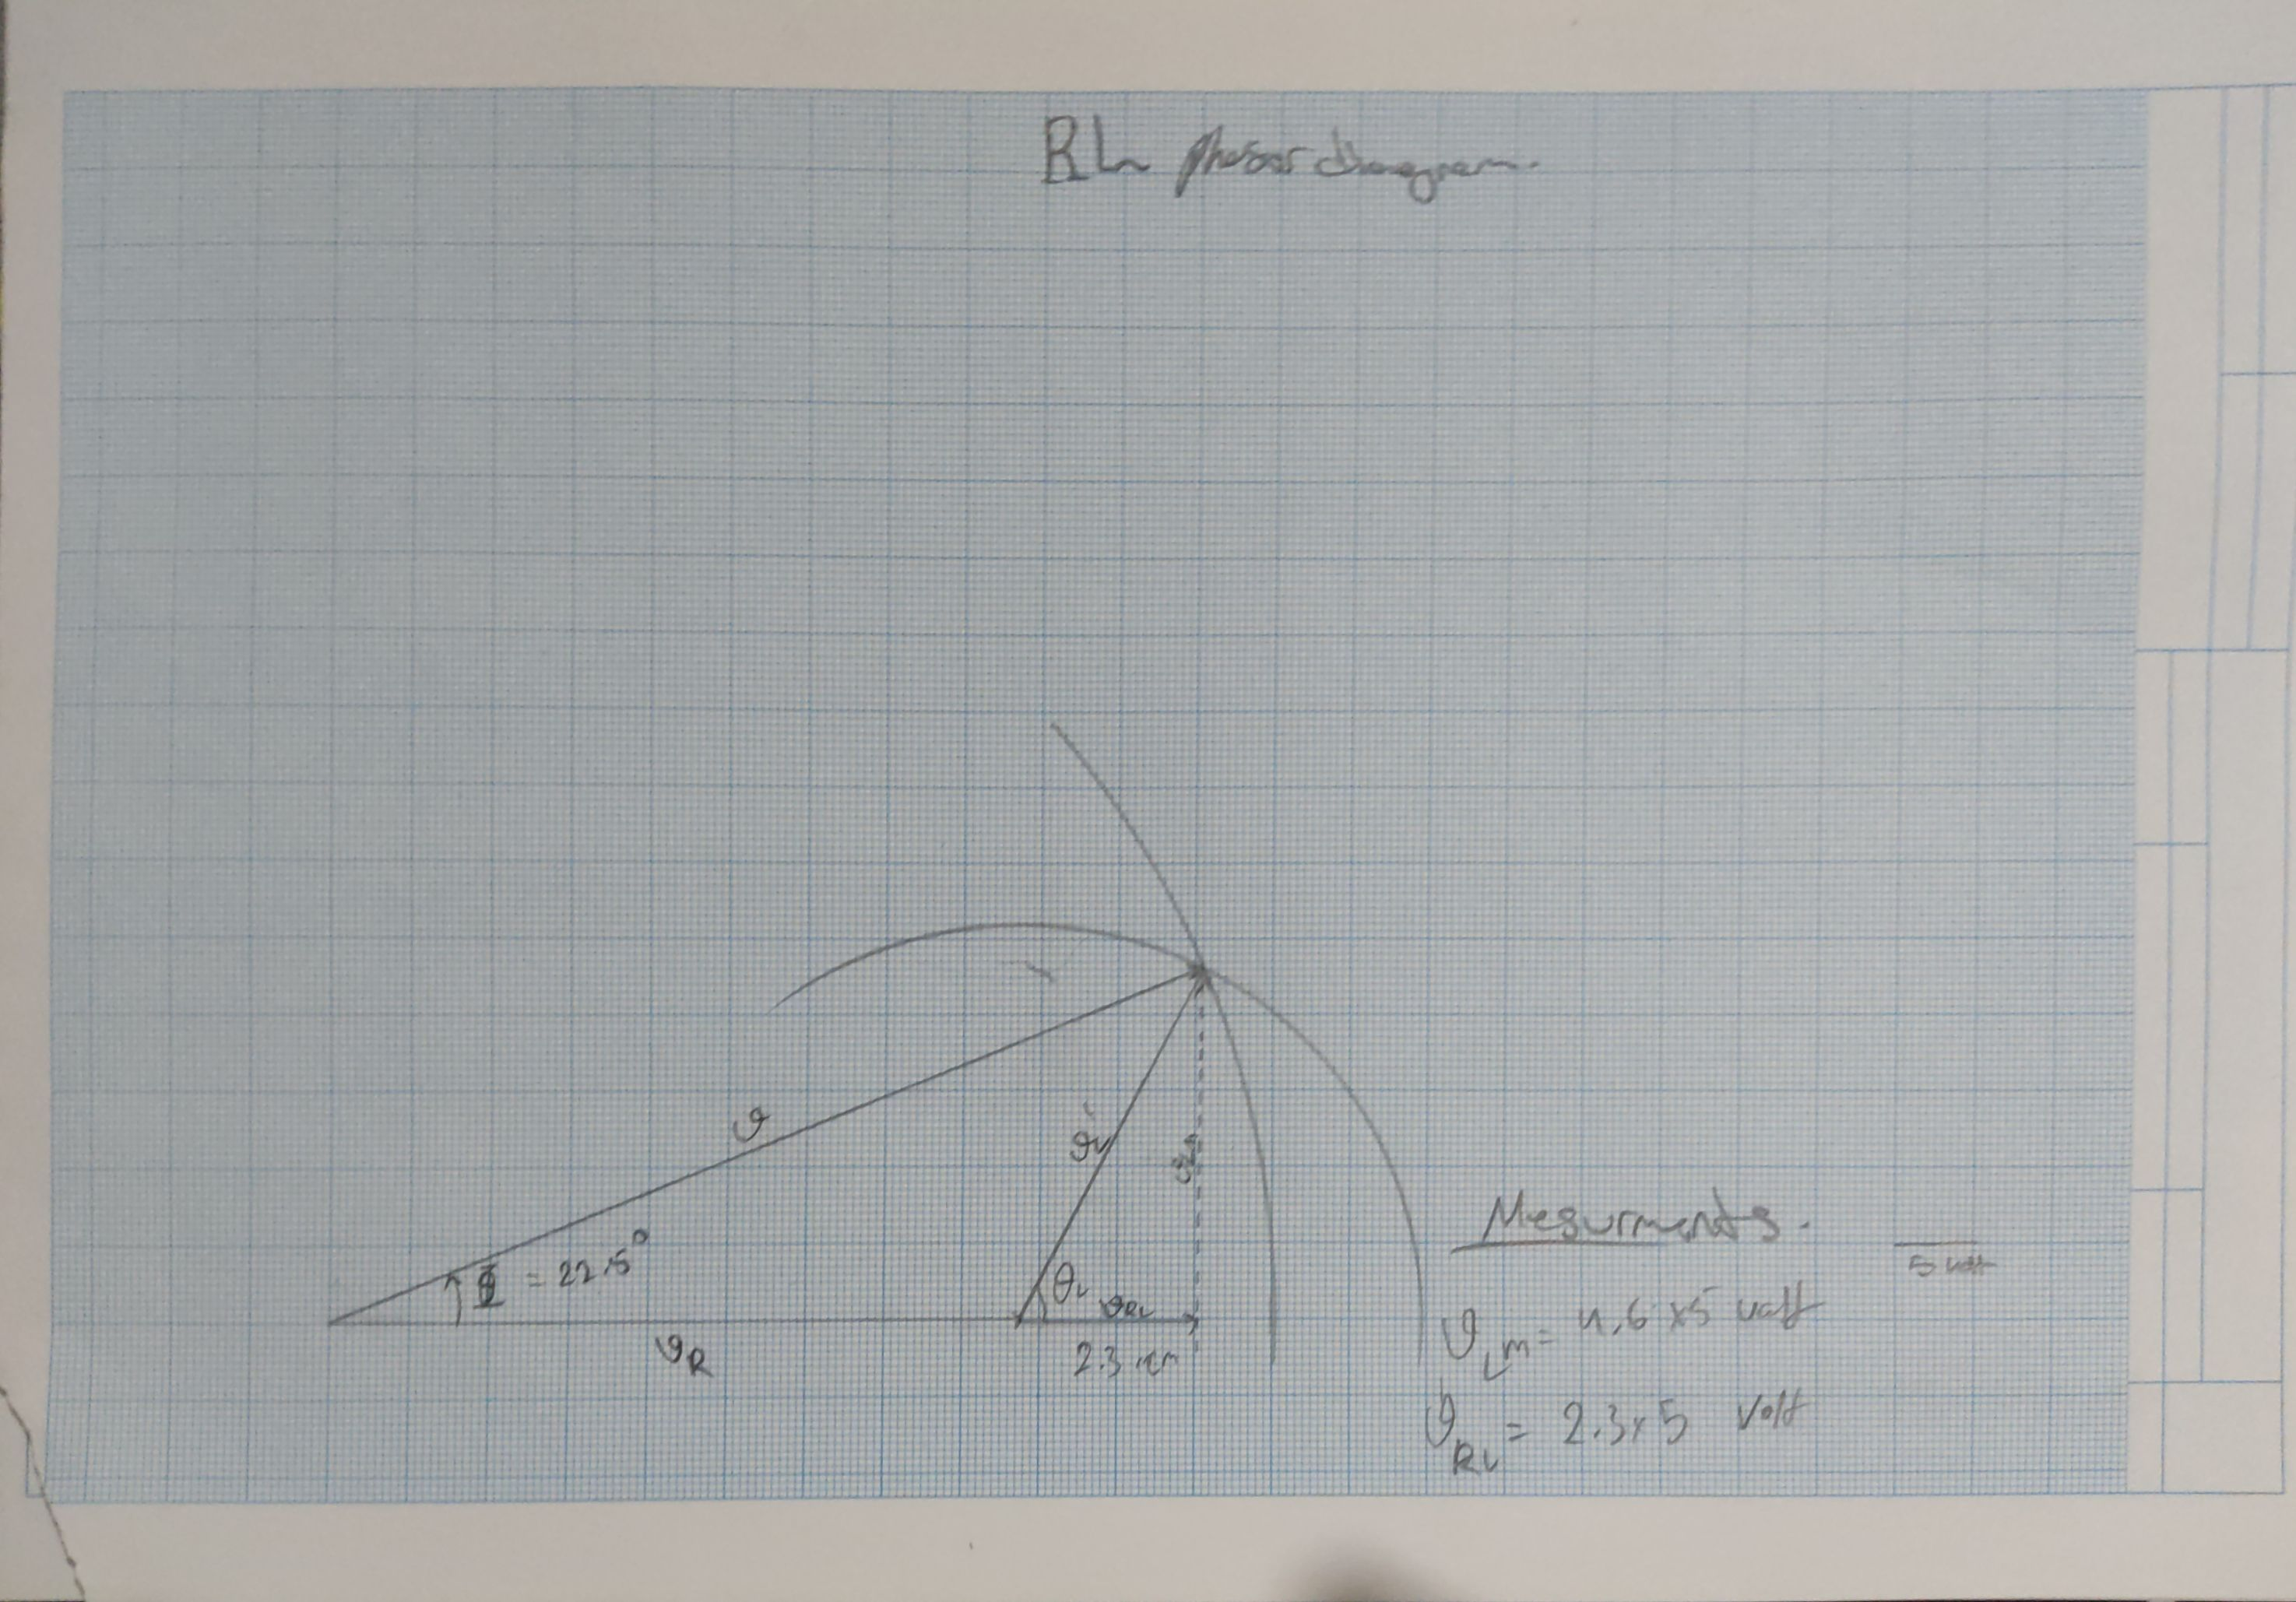
\includegraphics[width=\linewidth]{output_plots/phasor_diagram_rl.png}
    \caption{Phasor Diagram for RL Circuit}
    \label{fig:phasor_rl}
\end{figure}

\begin{figure}[H]
    \centering
    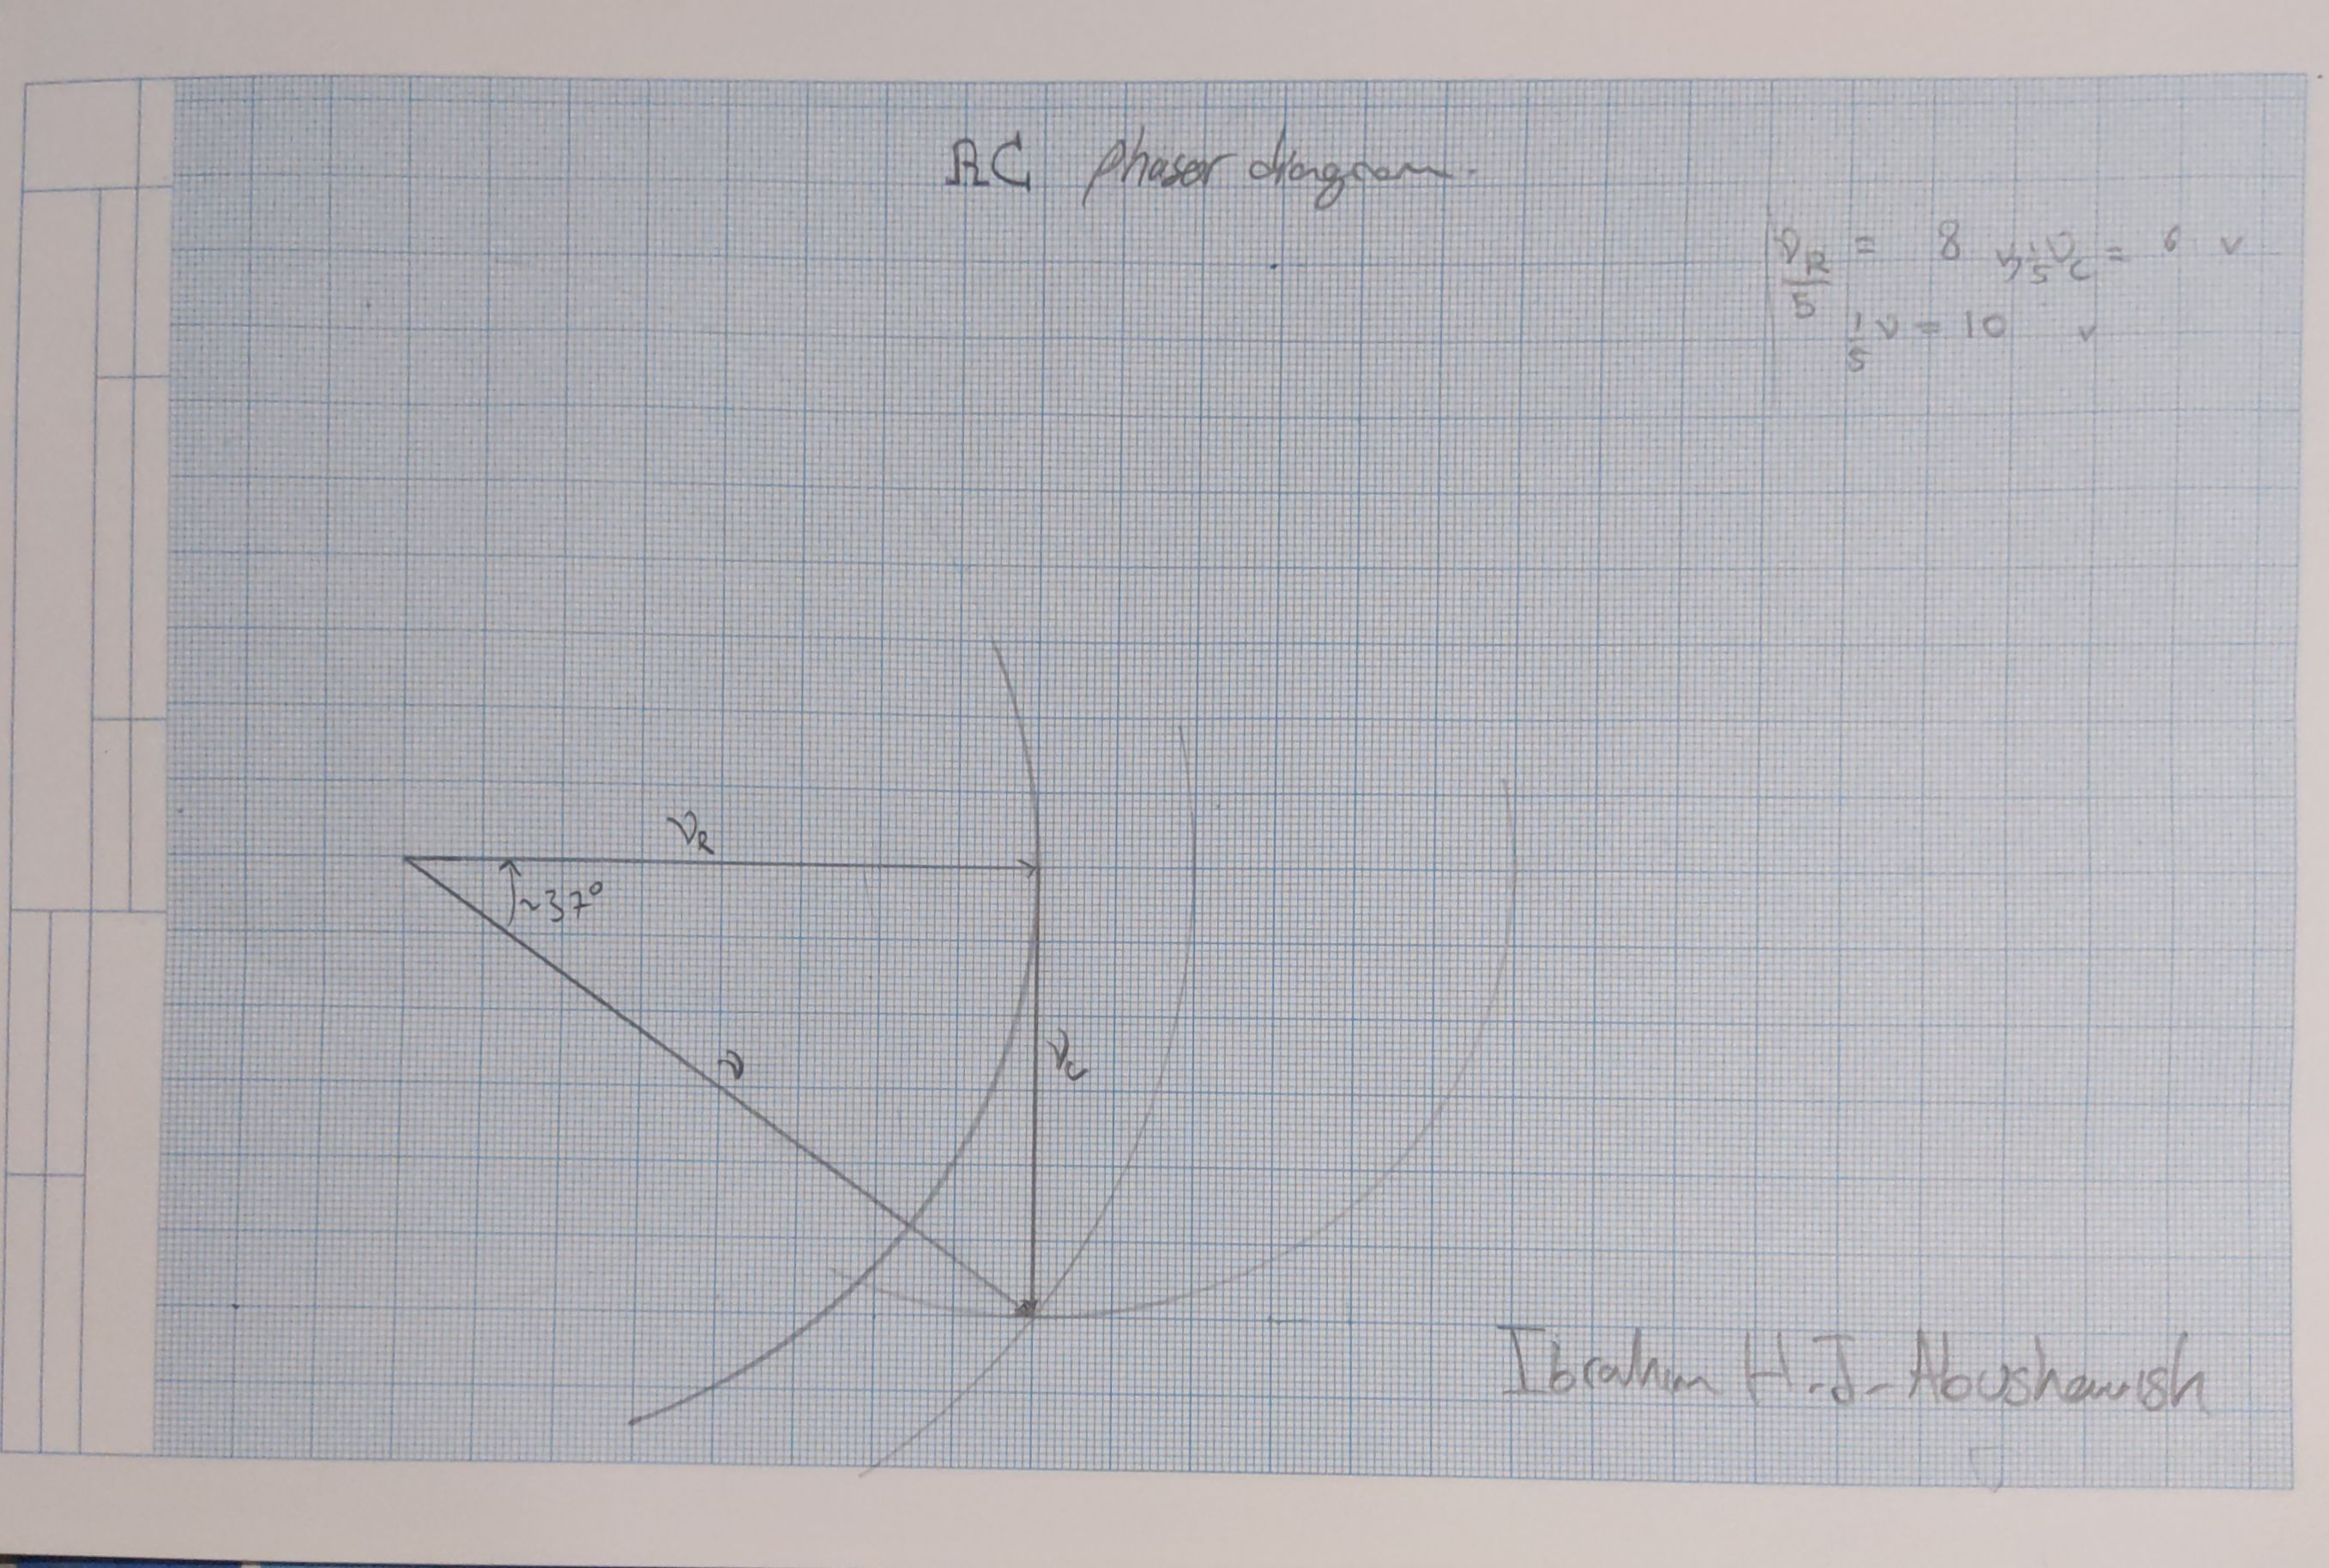
\includegraphics[width=\linewidth]{output_plots/phasor_diagram_rc.png}
    \caption{Phasor Diagram for RC Circuit}
    \label{fig:phasor_rc}
\end{figure}

% Discussion
\section{Discussion}
The phasor diagrams demonstrate the phase relationships between voltage and current in the RL and RC circuits. The RL circuit shows a phase shift where the current lags the voltage, while the RC circuit shows a phase shift where the current leads the voltage. These observations align with theoretical predictions.

In the RL circuit, the inductor causes the current to lag behind the voltage due to the inductive reactance, which increases with frequency. This behavior is evident from the phase angle \(\phi\) calculated in the results. The impedance of the RL circuit also increases with frequency, as shown by the impedance equation.

Conversely, in the RC circuit, the capacitor causes the current to lead the voltage due to the capacitive reactance, which decreases with frequency. The negative phase angle \(\phi_{RC}\) confirms this leading behavior. The impedance of the RC circuit decreases with increasing frequency, as indicated by the impedance equation.

The experimental results closely match the theoretical calculations, validating the accuracy of the experimental setup and measurement techniques. The variations in resistance and capacitance provided a comprehensive understanding of the circuit behavior under different conditions.

% Conclusion
\section{Conclusion}
This experiment highlights the principles of RL and RC circuits and demonstrates their behavior under different conditions. The experimental results confirm the theoretical relationships between resistance, inductance, capacitance, and circuit behavior.

The key findings include:
\begin{itemize}
    \item The RL circuit exhibits a phase shift where the current lags the voltage, with impedance increasing with frequency.
    \item The RC circuit shows a phase shift where the current leads the voltage, with impedance decreasing with frequency.
    \item The experimental data aligns well with theoretical predictions, validating the experimental methods used.
\end{itemize}

Understanding the behavior of RL and RC circuits is crucial for analyzing and designing electrical systems, particularly in applications involving signal processing and AC circuit analysis. The insights gained from this experiment provide a solid foundation for further studies in electrical engineering and related fields.

% Additional Resources
\section{Additional Resources}
For detailed information, including the Lab Manual, source code, and related experiments, visit the GitHub repository provided below or scan the QR code in Fig.~\ref{fig:qr_code}.

\begin{figure}[H]
    \centering
    \begin{minipage}{0.15\textwidth}
        \centering
        \qrcode[height=2cm]{https://github.com/ibeuler/LAB-Reports}
    \end{minipage}%
    \begin{minipage}{0.2\textwidth}
        \raggedright
        \caption{Access the GitHub repository for the lab manual, source code, and related experiments: \href{https://github.com/ibeuler/LAB-Reports}{\url{https://github.com/ibeuler/LAB-Reports}}.}
        \label{fig:qr_code}
    \end{minipage}
\end{figure}

\begin{thebibliography}{9}
\bibitem{lab_manual}
    ISTANBUL UNIVERSITY, \textit{Physics Laboratory II Experiment Book: Electricity and Magnetism}, Department of Physics, 2024.

\bibitem{github}
    \textit{Source code and additional experiments are available in the GitHub repository.} \url{https://github.com/ibeuler/LAB-Reports}
\end{thebibliography}

\end{document}